\section{Surface reconstruction}
Surface reconstruction from a large set of unstructured points obtained through laser scanning techniques or stereopsis is not a trivial task but nonetheless it is useful in many applications. For example a surface reconstruction could aid a robots end effector grasping some unknown object \cite{Wang2005}. Many methods for surface reconstruction exist in different domains of science, some algorithms are based on neural network approaches  \cite{Wu2007}, others are based on sculpting or region growing algorithms (e.g \cite{Bernardini1999} and \cite{Amenta2001}) used in computational geometry, some utilise an implicit method framework to represent incoming data as a surface \cite{Kazhdan2006} and \cite{Dong2011}.\\
\\
In 1999 F. Bernardini \textit{et al}. proposed in a fairly simple algorithm (Ball Pivoting Algorithm (BPA)) for reconstruction of surfaces from point clouds sampled over smooth objects \cite{Bernardini1999}. BPA is pivoting a sphere of a certain diameter around an edge of a seed triangle. Pivoting the sphere around all the edges is connecting three points to form a new triangle and so on. BPA is a part of the region growing algorithms as this algorithm uses a seed triangle builds the surface around this and outward. The algorithm is fairly easy to work with as it has one parameter which decides the radius of the sphere and that is it. N. Amenta \textit{et al}. proposed in 2001 \cite{Amenta2001} the power crust algorithm, which essentially is a three dimensional Voronoi approach \cite{Ledoux2007}. The power crust algorithm is well defined and proven which makes it one of the most known algorithm regarding surface reconstruction. This algorithm is a sculpting algorithm in computational geometry. Common for those algorithms mentioned is that these are explicit methods which requires neighboring information which leads to high computational time consumption. Therefore methods mentioned above are not well suited for reconstruction of large data sets.\\
\\
In 2006, M. Kazhdan \textit{et al}. proposed in \cite{Kazhdan2006} an algorithm which resides in the implicit method framework, this algorithm is called Poisson Surface Reconstruction (PSR). PSR is a fitting scheme that allow solving for the indicator function of the surface. It is shown in \cite{Kazhdan2006} this approach of fitting a surface resembles the Fast Fourier Transform (FFT). In \cite{Kazhdan2006} it is shown that the FFT approach requires five times as much space but is approximately double as fast while creating approximately the same number of triangles. The real advantage of the Poisson approach is that it is scalable and therefore does not rely on a uniform distribution of points and thus a higher degree of details can be reconstructed in areas where the point density is higher.\\
J. Manson \textit{et al}. did in 2008 propose a wavelet approach of the problem of reconstructing surfaces of large sets of unstructured points \cite{Manson2008}. The method is robust to noise in data because it is relying on implicit methods as PSR, and is therefore well-suited for reconstruction of real data which is overlayed with some random noise. The wavelet approach an advantages over PSR, the wavelet approach is able to reconstruct non-closed surfaces in opposition to PSR \cite{Kazhdan2006}. Using the Haar wavelet synthesise an acceptable surface if the points are well-aligned, else more smooth wavelets can be used such as Daubechies-2. Using octrees and small-support wavelets makes the synthesisation very fast, smaller support equals less computational time and space. Using Daubechies-2 compared to Haar increases computational time by a scale of four, and the space consumption is upscale by approximately four as well. As the methods for reconstruction mentioned first does not guarantee watertight mesh and does not work very well with large point sets, mean those methods are not of interest for further studies. The PSR and the wavelet approach both does estimate an indicator function of the surface, but each handles this indicator function differently. As these method is based on implicit methods they are more robust to noise in the input and approximates the surfaces better compared to the methods mentioned first.

\subsection{Overview of reconstruction scheme}
The wavelet method for surface reconstruction chosen for this custom implementation is highly inspired by the description in \cite{Manson2008}. One main reason for using wavelets for the analysis of the surface compared to more conventional methods like FFT is that wavelets support localisation in spatial and frequency(scale) domains. This mean that analysis is made locally instead of globally, which leads to the possibility of reconstructing finer details in input data, that would otherwise be hidden by the global analysis. PSR is approximating an indicator function\marginnote{ref: indicator function} of the surface by solving a Poisson equation\marginnote{ref: Poisson eq.}. In the wavelet approach an indicator function is also estimated, but the way it is done is different. The wavelet approach approximates the wavelet coefficients of the indicator function by making a Multi Resolution Analysis (MRA) of the input data\marginnote{ref: MRA, coeffs}. After the coefficients have been calculated the marching cube algorithm is utilised for triangulation of the surface, reconstructing the surface from the approximation of the indicator function.

\subsection{Wavelet coefficients} \marginnote{Could use some further description...}
In the method mentioned in \cite{Manson2008}, the indicator function of the surface $\partial M$ of an object $M$ is described as follows

\begin{equation}
	\chi_M(\textbf{x}) = 
	\begin{cases}
	1, & \textbf{x} \in M\\
	0, & elsewhere
	\end{cases} 
	\label{eq:indicator_fnc}
\end{equation}

\noindent The indicator function is defined as a set $\chi_M$ of $\textbf{x}$, being one if the $\textbf{x}$ is a part of the object $M$ else zero.\\
\\
Eq. \ref{eq:wavelet_coeffs} calculates an approximation of the wavelet coefficients of the indicator function $\chi_M$. For further details on the derivation of eq. \ref{eq:wavelet_coeffs} consult \cite{Manson2008}, parameters for the equation is shortly surveyed in the following.\\

\begin{equation}
	c^e_{j,\textbf{k}} \approx 2^{3j \over 2} \sum_{p_i \in \partial M \cap \textit{supp}(\psi^e_{j,\textbf{k}})} \vec{F}^e_{j,\textbf{k}} (p_i) \cdot \vec{n}_i d \sigma_i 
	\label{eq:wavelet_coeffs}
\end{equation}

\noindent Parameters $e$ is called the gender of the wavelet and describes a tensor of the basis being used, $j$ is the level at which the input data is analysed and $\textbf{k}$ is the translation of the wavelet basis itself. Parameters $p_i$ is a single point in the input data, $\partial M$ is the surface of $M$ and $\textit{supp}(\psi^e_{j,\textbf{k}})$ is denoting the support of the wavelet. The support of a wavelet is equal its boundaries. $\vec{F}^e_{j,\textbf{k}} (p_i)$ is a vector field of input data, or expressed differently, it is the volume density of the solid $M$. The parameter $\vec{n}_i$ is the outward unit normal to the surface $\partial M$ at point $p_i$. Last, $d \sigma_i$ denotes the differential surface of the surface $\partial M$, which is described by eq. \ref{eq:diff_area}.

\begin{equation}
	d \sigma_i = \frac{2^{-2 \cdot d_i}}{m},
	\label{eq:diff_area}
\end{equation}

\noindent where $d_i$ is the depth of the leaf in the oc-tree of the corresponding point $p_i$ and $m$ is the number of points in the current leaf.

\subsection{Marching cubes}\marginnote{Could use some further description...}
Marching cubes was proposed by W. E. Lorensen in 1987 in \cite{Lorensen:1987:MCH:37402.37422} and is utilised by the algorithm proposed in \cite{Manson2008}. The algorithm is using a conquer and divide approach to locate the surface inside a logical cube (a voxel), see figure \ref{fig:voxel}. The algorithm determines how the surface intersects with the voxel edges and then march to the next voxel. A one is assigned to the voxels vertex if the data at that vertex is exceeding the surface of interest.

\begin{figure}[htb]
	\begin{center}
		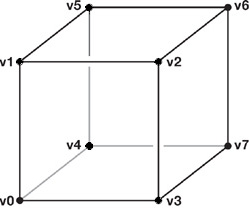
\includegraphics[scale=0.7,trim=0 0 0 0]{graphics/07_modelling/voxel.jpg}%trim=l b r t
		\caption{Illustrates a voxel.}
		\label{fig:voxel}
	\end{center}
\end{figure}

\noindent In each voxel there are eight vertices that leads to $2^8 = 256$ different combinations of surface inside the voxel, all these combinations can be reduced to fourteen patterns if the topology of all the patterns is taken into considerations, the fourteen patterns can be seen in figure \ref{fig:mc}. Complementary voxels amounts to one half of the full set of possible voxels while rotational symmetries 
reduces the number of unique voxels to fourteen.

\begin{figure}[htb]
	\begin{center}
		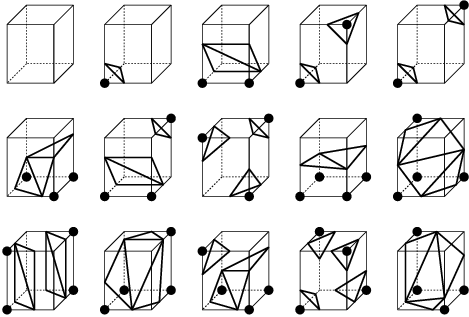
\includegraphics[scale=0.7,trim=0 0 0 0]{graphics/07_modelling/marchingcubes.png}%trim=l b r t
		\caption{Illustrates the different topologies of a voxel.}
		\label{fig:mc}
	\end{center}
\end{figure}

\noindent Using these different fourteen permutations of a voxel creates a watertight surface. \\
\\

\subsection{Implementation}\marginnote{No implementation yet...}
The surface reconstruction is implemented in ROS node making it compatible with the rest of the system. The assembled point cloud is passed from the filter node to the reconstruction node.


\subsection{Results}\marginnote{No results yet...}
